% !TeX encoding = UTF-8
% !TeX TS-program = xelatex

\documentclass[12pt,a4paper,final,twoside,fleqn]{book}
\newcommand{\bookauthor}{姜青娥}
\newcommand{\booktitleI}{数值分析及代码手册}
\newcommand{\booktitleII}{Cpp etc}
\newcommand{\booktitle}{\booktitleI{} \booktitleII}
\newcommand{\booksubtitle}{}
\newcommand{\bookinstitution}{克莱登大学}
\newcommand{\bookedition}{ImageNature}
\newcommand{\bookversion}{ver 1}
\newcommand{\bookkeywords}{Math}
\newcommand{\bookemail}{imagenature@proton.me}
\usepackage{mycode}
\linespread{1.25}\selectfont

\begin{document}
%\raggedbottom
%\maketitle
\frontmatter
\maketitle
\input{copyright}

\tableofcontents
\mainmatter
\chapter{Cpp 基础}
\label{cha:cpp-base}
%\thispagestyle{empty}

%% Calculate how old C is...
\newcount\cdifference\cdifference=\the\year\advance\cdifference by -1970

引用\cite{1989programming}

\begin{code}
  type 'a Process = 'a Signal IObservable
  type 'a Process = 'a Signal IObservable
\end{code}
\cs{love}

\cs{for (i=0; i<5; i++) if (i==0);for (i=0; i<5; i++) if (i==0)for (i=0; i<5; i++) \\ if (i==0)for (i=0; i<5; i++) if (i==0)for (i=0; i<5; i++) if (i==0)}


C is al een oude taal. De taal is rond 1970 ontworpen door Dennis Ritchie\footnote{Dennis MacAlister Ritchie (1941 -- 2011). Hij was de ontwerper van de programmeertaal C en was een van de ontwerpers van Unix. Bekende afgeleiden van Unix zijn Linux en FreeBSD.} en is dus al zo'n \the\cdifference\ jaar oud.

\begin{infobox}[{Bits and bytes{,} size does matter...}]
  De meeste gangbare computersystemen slaan data op in \textsl{bytes}. Een byte is een eenheid van~8 \textsl{bits}. Het woord \textsl{bit} is een samentrekking van \textsl{binary digit}. Binary digit betekent \textsl{binair cijfer} en binair betekent \textsl{tweewaardig}. Dat betekent dat een bit twee verschillende waarden kan hebben. We noemen die waarden 0 of 1. Met behulp van bits en bytes kunnen we getallen representeren. Het kleinste getal in een byte is 00000000$_2$ waarbij het subscript 2 aangeeft dat het om een binair getal gaat, en het grootste getal is 11111111$_2$. Het getal 00000000$_2$ komt overeen met het decimale getal 0 en 11111111$_2$ komt overeen met 255. Om grotere getallen te representeren, zijn meerdere bytes nodig. Moderne systemen kunnen \textsl{van nature} overweg met 32-bits eenheden, ze kunnen met 32 bits als één eenheid rekenen. Daarvoor zijn 4 bytes nodig. We spreken dan van een \textsl{32-bits systeem}. Daarnaast kunnen veel systemen ook overweg met 64-bits eenheden, dus zijn er 8 bytes nodig voor zo'n eenheid. We noemen dat\footnote{Een programmeerparadigma is een manier van programmeren en een wijze waarop een programma wordt vormgegeven.}. een \textsl{64-bits systeem}.
\end{infobox}

\begin{dosbox}[title=Een voorbeeld van een command line interface.,label=fig:commandlineint]
  C:\Users\Cbook> (*\textbf{notepad mooi.c}*) (*\hfill\textrm{(start Notepad)} *)
  C:\Users\Cbook> (*\textbf{gcc -o mooi.exe mooi.c}*) (*\hfill\textrm{(start C-compiler)}*)
  C:\Users\Cbook> (*\textbf{.\textbackslash mooi.exe}*) (*\hfill\textrm{(start uitvoerbaar programma)}*)
  C is een mooie taal (*\hfill\textrm{(de uitvoer op het scherm)}*)
  C:\Users\Cbook>
\end{dosbox}
Dit is echter niet de werkwijze van veel programmeurs. Gelukkig zijn er goede ontwikkelsystemen (IDE: Integrated Development Environment) die het programmeerwerk verlichten. Bekende systemen zijn Microsoft Visual Studio~\cite{vs2022}, Code::Blocks~\cite{codeblocks2020} en Apple's Xcode~\cite{xcode2020}.

Zulke ontwikkelsystemen zorgen ervoor dat de programmeur gemakkelijk het programma kan invoeren, de compiler kan starten en het programma kan \textsl{debuggen}\index{debuggen}. Dat laatste is vaak nodig als blijkt dat de executie van een programma niet verloopt zoals de programmeur het voor ogen had. Met debuggen wordt het programma stap voor stap doorlopen en kan de programmeur (of is het debugger) de inhoud van \textsl{variabelen}\index{variabele} bekijken. Ook kan de programmeur bepalen of de \textsl{statements}

 Een voorbeeld is te zien in figuur~\ref{fig:commandlineint}.


\begin{dosbox}[title=Een voorbeeld van een command line interface.,label=fig:commandlineint]
  C:\Users\Cbook> (*\textbf{notepad mooi.c}*) (*\hfill\textrm{(start Notepad)} *)
  C:\Users\Cbook> (*\textbf{gcc -o mooi.exe mooi.c}*) (*\hfill\textrm{(start C-compiler)}*)
  C:\Users\Cbook> (*\textbf{.\textbackslash mooi.exe}*) (*\hfill\textrm{(start uitvoerbaar programma)}*)
  C is een mooie taal (*\hfill\textrm{(de uitvoer op het scherm)}*)
  C:\Users\Cbook>
\end{dosbox}

\begin{dosbox}[title=Uitvoer van het programma in listing~\ref{cod:sumoftwo}.,label=fig:unuitvoerprog]
  Geef een getal: (*\textbf{7}*)
  Geef nog een getal: (*\textbf{4}*)
  De som van 7 en 4 is 11
\end{dosbox}
\begin{infobox}[To \texttt{scanf} or not to \texttt{scanf}...]
  \label{fig:unopmerkingscanf}%
  De Microsoft C-compiler bestempelt \texttt{scanf} als ``onveilig''. Een compilatie met \texttt{scanf} zal eindigen met een foutmelding. In plaats daarvan moet de functie \texttt{scanf\_s} worden gebruikt. Helaas ondersteunen andere compilers deze functie niet. Dat zal resulteren in een programma dat niet door iedere compiler kan worden vertaald. Om het probleem te omzeilen hebben we gebruik gemaakt van een \textsl{pragma}:

  \hspace*{1em}\texttt{\#pragma warning(disable : 4996)}

  We geven aan dat de C-compiler fout 4996 moet negeren. Op andere compilers, bijvoorbeeld de GNU-C compiler, wordt deze regel overgeslagen (er volgt wel een waarschuwing en met behulp van \textsl{conditionele compilatie} kan deze pragma overgeslagen worden). Overigens wordt op vele fora gewaarschuwd voor de onveiligheid van \texttt{scanf} en worden alternatieven gegeven. Wij gebruiken \texttt{scanf} hier wel \textsl{for the sake of simplicity}. Het is beter om \texttt{scanf} te vermijden.
\end{infobox}

\begin{figure}[!ht]
  \centering
  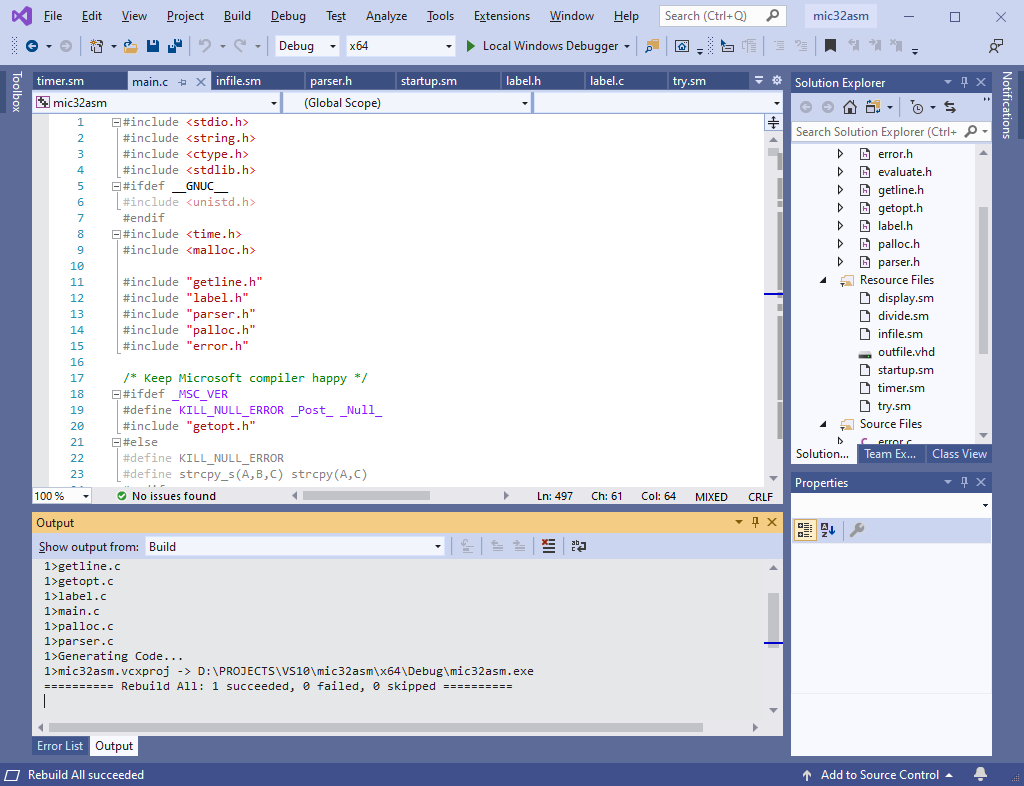
\includegraphics[width=\textwidth]{images/vs2019}
  \caption{Voorbeeld van Microsoft Visual Studio.}
  \label{fig:unvs2019}
\end{figure}
%\lipsum[1-5]

\begin{figure}[H]
  \begin{lstlisting}[caption=Een minimaal C-programma.,label=cod:unminimaalcprogramma]
    int main(void)
    {
      return 0;
    }
  \end{lstlisting}
\end{figure}


Het C-programma begint met de definitie van de \textsl{functie} \texttt{main}\indextwo{main}{functie}. Een functie is een aantal instructies samengepakt onder een gemeenschappelijke noemer. \textsl{Elk C-programma heeft een functie \texttt{main}}. Tussen de haken staat het keyword \texttt{void}\indexkeyword{void}, dat aangeeft dat het uitvoerbaar programma geen gegevens meekrijgt van het besturingssysteem\footnote{Dat kan wel, zie hoofdstuk~\ref{cha:pointers}.}. Vóór \texttt{main} staat het keyword \texttt{int}\indexkeyword{int} dat aangeeft dat \texttt{main} een geheel getal teruggeeft aan het besturingssysteem.





Binnen \texttt{main} zien we één \textsl{statement}\index{statement}. Een statement is een opdracht in de C-taal. Het statement wordt gevormd door het keyword \texttt{return}\indexkeyword{return} gevolgd door het getal 0 en een punt-komma. Bij uitvoering van dit statement wordt de waarde 0 teruggegeven aan het besturingssysteem. Dat behoeft enige uitleg. Een (gecompileerd) programma wordt gestart door het besturingssysteem. Aan het einde wordt het programma afgesloten. Het besturingssysteem ``ruimt'' het programma op en zorgt ervoor dat het gebruikte geheugen weer vrijgegeven wordt voor volgende programma's. We kunnen aan het besturingssysteem een getal teruggeven, in dit geval~0. Het is aan het besturingssysteem om hier wat mee te doen. Gebruikelijk is om 0 terug te geven als alles goed verlopen is. Een ander getal dan 0 geeft over het algemeen aan dat er iets fout gegaan is. Vanaf C99 is het niet meer nodig om dit \texttt{return}-statement uit te voeren. Dan wordt automatisch het getal 0 teruggegeven.



\begin{figure}[!ht]
  \begin{lstlisting}[caption=Afdrukken van de som van twee getallen.,label=cod:uneersteprogramma]
    #include <stdio.h>

    int main(void)
    {
      int a = 3;
      int b = 7;

      int som;

      som = a + b;

      printf("De som van %d en %d is %d\n", a, b, som);

      return 0;
    }
  \end{lstlisting}
\end{figure}

\begin{figure}
  \lstinputlisting[label=cod:uneerst,tabsize=4,language=c,caption={[Code2] An very important code}]{main.cpp}
\end{figure}

In regel 1 wordt een zogenoemd \textsl{header-bestand}\index{header-bestand} geladen, in dit geval het bestand \texttt{stdio.h}\indextwo{stdio.h}{header-bestand}. We leggen zo meteen uit waarom dat nodig is.

In regel 3 wordt kenbaar gemaakt dat het programma de functie \texttt{main}\indextwo{main}{functie} heeft. Een C-programma heeft \textsl{altijd} de functie \texttt{main}. Het (gecompileerde) programma wordt hier gestart. Het programma wordt gestopt na het laatste statement in \texttt{main}. Dit is per definitie een \mbox{\texttt{return}}-statement.

 dit geval \texttt{\textbackslash n}. Dit zorgt ervoor dat een volgende afdruk wordt begonnen aan het begin van de volgende rege

We kunnen het vorige programma interessanter maken door aan de gebruiker te vragen om twee gehele getallen in te voeren. Naast het afdrukken van tekst met de functie \texttt{printf} maken we nu ook gebruik van de functie \texttt{scanf}\indexfunc{scanf} om gehele getallen in te lezen. Het programma is te zien in listing~\ref{cod:sumoftwo}.

\booklistingfromproject[]{C}{Programma om de som van twee getallen te bepalen}{sumoftwo}{c}{!ht}

r op pagina~\pageref{fig:unopmerkingscanf}.


\section{Keywords}
In tabel~\ref{tab:unkeywords} is een lijst te zien met gereserveerde woorden. Een aantal van deze woorden hebben we al gezien zoals \texttt{int}, \texttt{void} en \texttt{return}. Deze woorden worden \textsl{keywords}\index{keyword} genoemd en vormen de vocabulaire van de taal C.

\begin{table}[!ht]
  \caption{Een lijst met keywords in de C-taal.}
  \label{tab:unkeywords}
  \centering\ttfamily
  \begin{tabular}{p{2.5cm}p{2.5cm}p{2.5cm}p{2.5cm}}
    \toprule
    auto &  double &  int & struct \\
    break & else  & long  &  switch \\
    case & enum & register & typedef \\
    char & extern & return & union \\
    const & float & short &  unsigned \\
    continue & for & signed & void \\
    default & goto & sizeof & volatile \\
    do & if & static & while \\
    \bottomrule
  \end{tabular}
\end{table}



Met behulp van de keywords \texttt{if}\indexkeyword{if} en \texttt{else}\indexkeyword{else} kunnen we in het programma beslissingen nemen op basis van een \textsl{conditie}\index{conditie}. Dit is te zien in listing~\ref{cod:unif}. We definiëren twee variabelen \texttt{a} en \texttt{b} en kennen gelijk de waarden
\begin{lstlisting}[style=lstoneline]
  unsigned long int a;
\end{lstlisting}

\begin{figure}[!b]
  \begin{lstlisting}[caption=Afdrukken van tekst op basis van een beslissing.,label=cod:unif]
    #include <stdio.h>

    int main(void)
    {
      int a = 7;
      int b = 9;

      if (a < b)
      {
        printf("a is kleiner dan b\n");
      }

      return 0;
    }
  \end{lstlisting}
\end{figure}


Technisch gezien hoort de \texttt{else} in regel 18 bij de \texttt{if} in regel 14. Let erop dat het vergelijken van \texttt{a} en \texttt{b} op gelijkheid in regel 12 een \textsl{dubbele is-gelijk-teken} (\texttt{==})\indexop{==} bevat.




\booklistingfromproject[]{C}{Afdrukken van de kwadraten van 1 t/m 10.}{printkwadraten}{c}{!ht}



\begin{figure}[!ht]
  \begin{lstlisting}[caption=Gebruik van een \texttt{for}-statement.,label=cod:unfor]
    for (getal = ondergrens; getal <= bovengrens;
    getal = getal + stap)
    {
      printf("Het kwadraat van %3d is %3d\n",
      getal, getal * getal);
    }
  \end{lstlisting}
\end{figure}

vergelijking~\eqref{equ:sqrtbab}.
%
\begin{equation}
  \label{equ:sqrtbab}
  \begin{split}
    x_0 &= S &&&& \text{beginsituatie} \\
    x_{n+1} &= \dfrac{1}{2}\cdot\left(x_n + \dfrac{S}{x_n}\right) &&&& \text{nieuwe situatie}\\
    \sqrt{S} &= \lim_{n\rightarrow\infty} x_n &&&& \text{uiteindelijke resultaat}
  \end{split}
\end{equation}


\begin{lstlisting}[caption=Voorbeeld van een string.]
  char str[] = "Ik ben een string";
\end{lstlisting}




\begin{lstlisting}[caption=Voorbeeld van een string.]
  char str[] = "Ik ben een string";
\end{lstlisting}

We hoeven de lengte van de string in dit geval niet op te geven, dat wordt automatisch door de C-compiler uitgerekend. Dat C functies heeft voor het afhandelen van string is te zien in listing~\ref{cod:intexamplestrlen}. In dit programma gebruiken we de functie \lstinline|strlen| (string length) om de lente van de string te bepalen. Wel moeten we het header-bestand \lstinline|string.h| laden waarin de stringfuncties gedeclareerd zijn.

\begin{lstlisting}[caption=Voorbeeld van een stringfunctie.,label=cod:intexamplestrlen]
  #include <stdio.h>
  #include <string.h>

  int main(void)
  {
    char string[] = "Ik ben een string";

    int len = strlen(string);

    printf("De lengte is %d\n", len);

    return 0;
  }
\end{lstlisting}

Strings worden behandeld in hoofdstuk~\ref{cha:arrays}.

\begin{figure}[!ht]
  \begin{lstlisting}[caption=K\&R-stijl.]
    while (a < b) {
      (*\normalfont\textsl{statements}*)
      if (a < 0) {
        (*\normalfont\textsl{statements}*)
      }
    }
  \end{lstlisting}

\end{figure}
In de Allman-stijl\index{Allman-stijl} wordt de accolade-openen \textsl{onder} een functie, beslissings- of herhalingstatement geschreven. De statement hierbinnen worden \textsl{ingesprongen}. Bij gebruik van in elkaar verweven beslissings- of herhalingstatement worden de statement verder of dieper ingesprongen.

\begin{lstlisting}[caption=Allman-stijl.]
  if (a < b)
  {
    if (a < 0)
    {
      (*\normalfont\textsl{statements}*)
    }
  }
\end{lstlisting}












\blinddocument
%\chapter{Cpp 基础}
\label{cha:cpp-base}
%\thispagestyle{empty}

%% Calculate how old C is...
\newcount\cdifference\cdifference=\the\year\advance\cdifference by -1970

C is al een oude taal. De taal is rond 1970 ontworpen door Dennis Ritchie\footnote{Dennis MacAlister Ritchie (1941 -- 2011). Hij was de ontwerper van de programmeertaal C en was een van de ontwerpers van Unix. Bekende afgeleiden van Unix zijn Linux en FreeBSD.} en is dus al zo'n \the\cdifference\ jaar oud. Hij was bezig met het schrijven van een besturingssysteem (Engels: operating system)\footnote{Een besturingssysteem is een programma dat draait op een computer en zorgt voor het beschikbaar stellen van \textsl{resources} aan de gebruiker (lees: programma's). Zo zorgt een besturingssysteem ervoor dat de bestanden op de harde schijf netjes worden opgeslagen en beschikbaar zijn. Daarnaast zorgt een besturingssysteem ervoor dat programma's netjes naast elkaar kunnen draaien. Drie bekende besturingssystemen zijn Windows, Linux en Apple's OS-X.} en zocht naar een mogelijkheid om dit te schrijven op een hoger niveau dan gebruikelijk was voor die tijd. In die tijd werden besturingssystemen geschreven in assembly, een taal die dicht bij de hardware van de computer ligt. Programma's schrijven in assembly is tijdrovend en gevoelig voor fouten van de programmeur.

C is een zogenoemde derde-generatietaal (3GL) en zorgt ervoor dat programma's gestructureerd kunnen worden geschreven zonder dat de programmeur kennis hoeft te hebben van de hardware waarop het programma draait. Toch biedt de taal constructies om die hardware in te stellen, een voorwaarde voor het schrijven van een besturingssysteem. Daarom is de taal geliefd bij programmeurs van kleine computersystemen waarop geen besturingssysteem draait, de zogenoemde \textsl{bare metal systems}\index{bare metal system}. Het is vaak ook de enige taal die gebruikt kan worden op dit soort systemen, naast assembly.

C is geschreven voor ervaren programmeurs die behoefte hebben aan het schrijven van compacte programma’s. Dat is te zien aan de soms onduidelijke taalconstructies. C is daarom lastig voor beginnende programmeurs. Maar het is, zoals gezegd, vaak de enige taal die op een een bepaald platform gebruikt kan worden en met enige discipline kan ook de minder ervaren programmeur de taal prima gebruiken.

C is een algemeen bruikbare taal (\textsl{general purpose language}) en is dus niet voor een specifiek doeleind ontworpen (behalve voor het schrijven van besturingssystemen). Zo kunnen met C wiskundige berekeningen worden uitgevoerd maar de programmeur moet zelf alles schrijven. Er zijn wel \textsl{functies} beschikbaar voor bijvoorbeeld sinus, cosinus en tangens. Er zijn echter talen die dit veel beter ondersteunen. Ook het verwerken van bestanden en \textsl{strings} (een rij karakters) is mogelijk maar dat moet door de programmeur zelf worden uitgewerkt. Ook hier zijn diverse functies beschikbaar die het programmeerwerk enigszins verlichten.

C is een \textsl{imperatieve} programmeertaal, een van de bekende programmeerparadigma's\footnote{Een programmeerparadigma is een manier van programmeren en een wijze waarop een programma wordt vormgegeven.}.


Een computer heeft naast de processor \textsl{geheugen}\index{geheugen} om de data en instructies op te slaan. Er zijn twee soorten geheugens: ROM\index{ROM} (Read Only Memory) is geheugen waarvan de inhoud niet gewijzigd kan worden; RAM\index{RAM} (Random Access Memory) is geheugen waarvan de inhoud wel gewijzigd kan worden. We zullen zo meteen zien waarvoor ROM en RAM worden gebruikt.

\begin{infobox}[{Bits and bytes{,} size does matter...}]
De meeste gangbare computersystemen slaan data op in \textsl{bytes}. Een byte is een eenheid van~8 \textsl{bits}. Het woord \textsl{bit} is een samentrekking van \textsl{binary digit}. Binary digit betekent \textsl{binair cijfer} en binair betekent \textsl{tweewaardig}. Dat betekent dat een bit twee verschillende waarden kan hebben. We noemen die waarden 0 of 1. Met behulp van bits en bytes kunnen we getallen representeren. Het kleinste getal in een byte is 00000000$_2$ waarbij het subscript 2 aangeeft dat het om een binair getal gaat, en het grootste getal is 11111111$_2$. Het getal 00000000$_2$ komt overeen met het decimale getal 0 en 11111111$_2$ komt overeen met 255. Om grotere getallen te representeren, zijn meerdere bytes nodig. Moderne systemen kunnen \textsl{van nature} overweg met 32-bits eenheden, ze kunnen met 32 bits als één eenheid rekenen. Daarvoor zijn 4 bytes nodig. We spreken dan van een \textsl{32-bits systeem}. Daarnaast kunnen veel systemen ook overweg met 64-bits eenheden, dus zijn er 8 bytes nodig voor zo'n eenheid. We noemen dat een \textsl{64-bits systeem}.
\end{infobox}

Naast ROM en RAM heeft de computer nog invoer- en uitvoermogelijkheden, anders is er geen communicatie met de buitenwereld mogelijk. De verzamelnaam is \textsl{I/O}\index{I/O} dat ``Input'' en ``Output'' betekent. Het is best lastig om de invoer en uitvoer te realiseren. Daarom wordt bij de gangbare computers een stuk software geladen (of het is al aanwezig in de ROM) om dat voor de gebruiker (en programmeur) te vereenvoudigen. Die software wordt een \textsl{besturingssysteem}\index{besturingssyteem} genoemd, maar gangbaar is om de Engelse naam \textsl{operating system}\index{operating system} te gebruiken. Bekende besturingssytemen zijn Windows, Linux en Apple's macOS.

Niet alle gegevens zijn in het geheugen van de computer aanwezig. Een computer heeft (vaak) \textsl{secundair geheugen}\index{secundair geheugen}. Voorbeelden van secundair geheugen zijn harddisk (harde schijf), USB-sticks en SD-cards. De informatie op deze geheugendragers blijft aanwezig ook al wordt de computer uitgezet en weer aangezet. Om de informatie beschikbaar te maken worden de gegevens in \textsl{bestanden}\index{bestand} (Engels: files) gezet. De manier waarop dat wordt gerealiseerd wordt een \textsl{bestandssysteem}\index{bestandssysteem} (Engels: file system) genoemd. Bekende bestandssystemen zijn NTFS op Windows en ext3 op Linux. Het besturingssysteem zorgt ervoor dat de bestanden op ordentelijke wijze kunnen worden benaderd.

In de praktijk komen we een drietal computersystemen tegen. Natuurlijk zijn er de algemeen bruikbare computers waarop een besturingssysteem draait (PC, laptops met Windows, Linux, Apple's macOS) en die een grote hoeveelheid aan verschillende programma's kan uitvoeren.

Daarnaast zijn er zogenoemde \textsl{embedded systems}\index{embedded system}. Een embedded system in meestal geschikt om één taak uit te voeren en is voorzien van een kleine processor met geheugen en I/O-faciliteiten. Al deze componenten zijn op één ic (Integrated Circuit of chip genoemd)\index{chip} geplaatst. We noemen zo'n processorsysteem een \textsl{microcontroller}\index{microcontroller}. Voorbeelden van embedded systems zijn (de besturingen van) wasmachines, koelkasten, televisies, thermostaten, horloges en bloeddrukmeters. De markt voor embedded systems is trouwens vele malen groter dan de markt voor algemeen bruikbare computers.
De microcontroller heeft meestal geen besturingssysteem. Dat noemen we \textsl{bare metal}\index{bare metal system} systemen. Dat betekent dat de programmeur alles zelf moet ontwikkelen. Gelukkig leveren fabrikanten kant-en-klare ontwikkelsystemen om programma's voor microcontrollers te produceren. Op deze systemen is C (en C++) de enige taal die gebruikt kan worden. We gaan in dit boek hier verder niet op in.

We kunnen natuurlijk niet de \textsl{smartphones} vergeten. Zo'n beetje iedereen in Nederland heeft er een. We kunnen een smartphone vergelijken met een algemeen bruikbaar computersysteem, waarop de besturingssystemen Android of iOS draaien. Op deze systemen kunnen programma's worden geïnstalleerd, \textsl{apps} genaamd. Deze apps worden over het algemeen \textsl{niet} in C geprogrammeerd, en vallen verder buiten het bestek van dit boek.

Bij PC's en laptops is een klein programma in ROM aanwezig. Dit zorgt ervoor dat de PC kan opstarten. Het heeft tot doel om het besturingssysteem te laden (Windows, Linux). Het besturingssysteem en de programma's worden dus in RAM geladen, net als de data waarmee de programma's werken. Op smartphones is het besturingssysteem opgeslagen in ROM die herprogrammeerbaar is. Zo kunnen updates van het besturingssysteem geïnstalleerd worden. De apps en data worden geladen in de RAM. Bij microcontrollers is het complete programma geladen in ROM, die ook herprogrammeerbaar is. De data is geplaatst in RAM.

% Dat worden \textsl{compiler suites} of \textsl{toolchains}\index{toolchain} genoemd.


\section{De compiler}
C is een zogenoemde derde-generatie-taal. De broncode van een C-programma is voor een mens gewoon te lezen. Deze broncode kan niet direct door de processor worden uitgevoerd. De \textsl{C-compiler}\index{compiler} vertaalt de broncode naar instructies die de processor wel kan uitvoeren. Dat vertalen wordt \textsl{compileren}\index{compileren} genoemd. De instructies worden in bitpatronen in het geheugen opgeslagen. De bitpatronen noemen we \textsl{machinecode}\index{machinecode}. Elk type processor heeft zijn eigen verzameling bitpatronen, dat wordt de \textsl{Instruction Set Architecture}\index{ISA} genoemd. De ISA van een Intel-processor is dus anders dan die van een ATmega-processor, maar we kunnen wel zeggen dat elke processor ongeveer dezelfde soort instructies bevat. De C-compiler moet weten voor welke processor een C-programma wordt vertaald.

Een C-programma kan niet worden uitgevoerd door de computer. We moeten eerst een programma compileren zodat instructies worden gegenereerd die de processor wel kan uitvoeren. De verzameling programma's om een C-programma te compileren wordt een \textsl{toolchain}\index{toolchain} genoemd. Het vertaalde programma wordt een \textsl{uitvoerbaar bestand}\index{uitvoerbaar bestand} of \textsl{executable}\index{executable} genoemd. Een uitvoerbaar bestand wordt net als een C-programma opgeslagen op de \textsl{vaste schijf} (SSD, USB-stick, $\ldots$). Bij het ontwikkelen van programma's voor microcontrollers wordt gebruik gemaakt van PC of laptop met een besturingssysteem en een C-compiler specifiek voor de microcontroller. We noemen zo'n compiler een \textsl{cross compiler}\index{cross compiler}. De uitvoerbare instructies worden via de PC in het geheugen van de microcontroller \textsl{geprogrammeerd}\index{programmeren}.






\section{Ontwikkelsystemen}
De meeste boeken gaan uit van een \textsl{command line interface} op een Unix-derivaat. Met behulp van een \textsl{editor} wordt een programma ingevoerd en wordt op de commandoregel de C-compiler gestart. Daarna wordt het programma (ook via de commandoregel) gestart.
Natuurlijk is het ook mogelijk om alles met behulp van de command line te doen. Deze werkwijze wordt veel gebruikt op Linux-systemen maar kan ook op Windows worden gebruikt. Een voorbeeld is te zien in figuur~\ref{fig:commandlineint}.

\begin{dosbox}[title=Een voorbeeld van een command line interface.,label=fig:commandlineint]
C:\Users\Cbook> (*\textbf{notepad mooi.c}*) (*\hfill\textrm{(start Notepad)} *)
C:\Users\Cbook> (*\textbf{gcc -o mooi.exe mooi.c}*) (*\hfill\textrm{(start C-compiler)}*)
C:\Users\Cbook> (*\textbf{.\textbackslash mooi.exe}*) (*\hfill\textrm{(start uitvoerbaar programma)}*)
C is een mooie taal (*\hfill\textrm{(de uitvoer op het scherm)}*)
C:\Users\Cbook>
\end{dosbox}

Dit is echter niet de werkwijze van veel programmeurs. Gelukkig zijn er goede ontwikkelsystemen (IDE: Integrated Development Environment) die het programmeerwerk verlichten. Bekende systemen zijn Microsoft Visual Studio~\cite{vs2022}, Code::Blocks~\cite{codeblocks2020} en Apple's Xcode~\cite{xcode2020}.
Zulke ontwikkelsystemen zorgen ervoor dat de programmeur gemakkelijk het programma kan invoeren, de compiler kan starten en het programma kan \textsl{debuggen}\index{debuggen}. Dat laatste is vaak nodig als blijkt dat de executie van een programma niet verloopt zoals de programmeur het voor ogen had. Met debuggen wordt het programma stap voor stap doorlopen en kan de programmeur (of is het debugger) de inhoud van \textsl{variabelen}\index{variabele} bekijken. Ook kan de programmeur bepalen of de \textsl{statements}\index{statement} (opdrachten voor de computer) op de juiste volgorde worden uitgevoerd.

Een voorbeeld van Microsoft Visual Studio is te zien in figuur~\ref{fig:unvs2019}. Visual Studio ondersteunt het ontwikkelen van software voor Windows-computers met behulp van een groot aantal talen: C, C++, C\#, Python. Het is zelfs mogelijk om software te ontwikkelen voor Linux-systemen. Een korte introductie wordt gegeven in bijlage~\ref{cha:visualstudio}.

\begin{figure}[!ht]
\centering
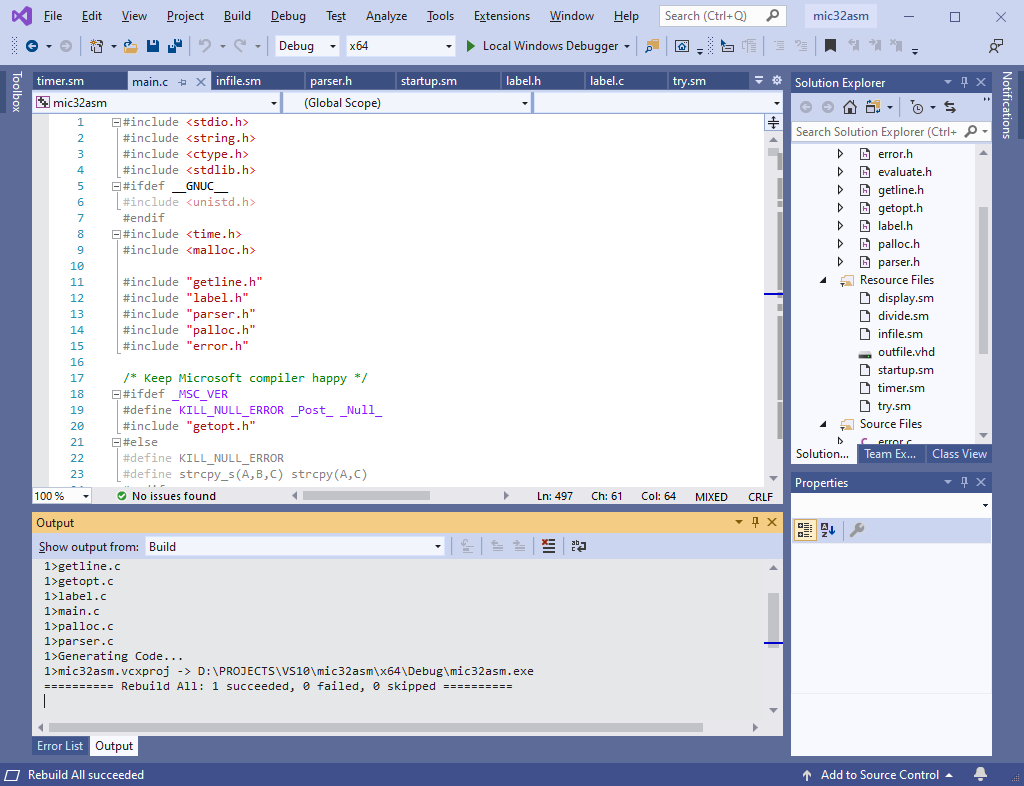
\includegraphics[width=\textwidth]{images/vs2019}
\caption{Voorbeeld van Microsoft Visual Studio.}
\label{fig:unvs2019}
\end{figure}

We hebben nu een beeld van hoe op een computer een C-programma wordt vertaald naar instructies voor een computer. De computer kan het C-programma niet direct uitvoeren, het programma moet gecompileerd worden. Als we een wijziging in het C-programma willen doorvoeren, dan moeten we het C-programma uiteraard opnieuw compileren.

We zullen in de overige paragrafen in sneltreinvaart enkele concepten van C behandelen. In de volgende hoofdstukken wordt de taal verder uitgediept.


\section{Een minimaal C-programma}
We beginnen met het meest simpele C-programma dat mogelijk is. We willen hiermee uitleggen wat er gebeurt als dit programma gecompileerd en uitgevoerd wordt. Het programma is te zien in listing~\ref{cod:unminimaalcprogramma}. Het programma doet in feite helemaal niets, althans niet dat de gebruiker van het programma kan waarnemen. Toch gebeuren er wel degelijk dingen `onder de motorkap'.

\begin{figure}[H]
\begin{lstlisting}[caption=Een minimaal C-programma.,label=cod:unminimaalcprogramma]
int main(void)
{
	return 0;
}
\end{lstlisting}
\end{figure}

Dit programma kan niet direct door de computer worden uitgevoerd, het moet eerst worden gecompileerd. Na compilatie is een \textsl{uitvoerbaar bestand}\index{uitvoerbaar bestand} beschikbaar dat wel door de computer kan worden uitgevoerd. De werking op een PC of laptop is als volgt. Als het uitvoerbare programma wordt gestart, dan zal het besturingssysteem het uitvoerbare programma in het geheugen van de computer laden. Dus ergens in het geheugen van de computer liggen de instructies die het programma vormen opgeslagen. Het besturingssysteem start het uitvoerbare programma door de processor naar de eerste instructie van het programma te leiden. Het programma (dat is het uitvoerbare programma) zal nu instructies uitvoeren. Na afloop van het programma wordt de besturing weer teruggeven aan het besturingssysteem.

Het C-programma begint met de definitie van de \textsl{functie} \texttt{main}\indextwo{main}{functie}. Een functie is een aantal instructies samengepakt onder een gemeenschappelijke noemer. \textsl{Elk C-programma heeft een functie \texttt{main}}. Tussen de haken staat het keyword \texttt{void}\indexkeyword{void}, dat aangeeft dat het uitvoerbaar programma geen gegevens meekrijgt van het besturingssysteem\footnote{Dat kan wel, zie hoofdstuk~\ref{cha:pointers}.}. Vóór \texttt{main} staat het keyword \texttt{int}\indexkeyword{int} dat aangeeft dat \texttt{main} een geheel getal teruggeeft aan het besturingssysteem.

Statements die in het C-programma gebruikt worden, zijn afgebakend met \textsl{accolades}\index{accolades}. Het Engelse woord hiervoor is \textsl{curly braces} of gewoon \textsl{braces}. De accolades geven het begin en einde aan van \textsl{blok}. Een blok begint met een accolade-openen (\texttt{\{}) en eindigt met een accolade-sluiten (\texttt{\}}). Over de plaats van de accolades zijn er diverse meningen. In listing~\ref{cod:unminimaalcprogramma} is de accolade-openen geplaatst onder de definitie van \texttt{main}, maar het is ook gebruikelijk om de accolade-openen te schrijven achter de definitie van \texttt{main}.

Binnen \texttt{main} zien we één \textsl{statement}\index{statement}. Een statement is een opdracht in de C-taal. Het statement wordt gevormd door het keyword \texttt{return}\indexkeyword{return} gevolgd door het getal 0 en een punt-komma. Bij uitvoering van dit statement wordt de waarde 0 teruggegeven aan het besturingssysteem. Dat behoeft enige uitleg. Een (gecompileerd) programma wordt gestart door het besturingssysteem. Aan het einde wordt het programma afgesloten. Het besturingssysteem ``ruimt'' het programma op en zorgt ervoor dat het gebruikte geheugen weer vrijgegeven wordt voor volgende programma's. We kunnen aan het besturingssysteem een getal teruggeven, in dit geval~0. Het is aan het besturingssysteem om hier wat mee te doen. Gebruikelijk is om 0 terug te geven als alles goed verlopen is. Een ander getal dan 0 geeft over het algemeen aan dat er iets fout gegaan is. Vanaf C99 is het niet meer nodig om dit \texttt{return}-statement uit te voeren. Dan wordt automatisch het getal 0 teruggegeven.


\section{Afdrukken op het scherm}
We kunnen het eerste programma interessanter maken door een regel tekst op het scherm af te drukken. Het programma in listing~\ref{cod:uneersteprogramma} drukt de regel \texttt{De som van 3 en 7 is 10} op het scherm af. We zullen het programma stap voor stap doorlopen.

\begin{figure}[!ht]
\begin{lstlisting}[caption=Afdrukken van de som van twee getallen.,label=cod:uneersteprogramma]
#include <stdio.h>

int main(void)
{
    int a = 3;
    int b = 7;

    int som;

    som = a + b;

	printf("De som van %d en %d is %d\n", a, b, som);

	return 0;
}
\end{lstlisting}
\end{figure}

\begin{figure}
  \lstinputlisting[label=cod:uneerst,tabsize=4,language=c,caption={[Code2] An very important code}]{main.cpp}
\end{figure}

In regel 1 wordt een zogenoemd \textsl{header-bestand}\index{header-bestand} geladen, in dit geval het bestand \texttt{stdio.h}\indextwo{stdio.h}{header-bestand}. We leggen zo meteen uit waarom dat nodig is.

In regel 3 wordt kenbaar gemaakt dat het programma de functie \texttt{main}\indextwo{main}{functie} heeft. Een C-programma heeft \textsl{altijd} de functie \texttt{main}. Het (gecompileerde) programma wordt hier gestart. Het programma wordt gestopt na het laatste statement in \texttt{main}. Dit is per definitie een \mbox{\texttt{return}}-statement.

In regel 5 en 6 worden twee \textsl{variabelen}\index{variabele} gedefinieerd, de variabelen \texttt{a} en \texttt{b}. Technisch gezien is een variabele een plek in het geheugen van de computer. Een variabele kan door het programma gebruikt worden om gegevens te bewerken. Definitie\index{definitie} wil zeggen dat een variabele kenbaar wordt gemaakt én dat er geheugenruimte wordt gereserveerd. Bij de definitie wordt opgegeven wat het type is van de variabele. Dit gebeurt middels het keyword \texttt{int}, dat betekent dat \texttt{a} en \texttt{b} alleen gehele getallen kunnen opslaan (Engels: integer). Aan de variabelen worden gelijk waarden toegekend. We noemen dit \textsl{initialisatie}\index{initialisatie} van variabelen.

%%%\begin{infobox}[Definitie versus declaratie]
%%%Bij programmeertalen wordt twee termen gebruikt: definitie en declaratie. Een definitie van een variabele is het kenbaar maken van een variabele en het reserveren van geheugenruimte op het moment van definiëren. Declaratie wil zeggen dat de variabele op een andere plek in het programma is gedefinieerd en dat het vanaf het punt van declaratie kan worden gebruikt.
%\end{infobox}

In regel 8 wordt de variabele \texttt{som} gedefinieerd zonder initialisatie. Dat betekent dat op dat moment de waarde (of inhoud) van de variabele \textsl{onbekend} is. Vervolgens wordt in regel 10 de som van \texttt{a} en \texttt{b} berekend middels de \textsl{optel-operator} \texttt{+}\indextwo{+}{optellen} en wordt het resultaat \textsl{toegekend}\index{toekenning}\indextwo{=}{toekennen} aan variabele \texttt{som}. Vanaf regel 10 is de waarde van \texttt{som} dus 10. In regel 10 zien we zogenoemde \textsl{expressies}\index{expressie}. Zo is \texttt{a + b} een expressie en is de toekenning \mbox{\texttt{som = ...}} ook een expressie. De term expressie komt veel voor in C.

In regel 12 wordt de functie \texttt{printf}\indexfunc{printf} aangeroepen. Deze functie is al geschreven en zit in de standard library. De functie krijgt vier \textsl{argumenten}\index{argument} mee, gegevens die in de functie verwerkt worden. Het eerste argument is een \textsl{string}\index{string}. Een string is een stukje tekst, maar we spreken ook wel van een rij karakters. Daarna volgen de (waarden) van de variabelen \texttt{a}, \texttt{b} en \texttt{som}.

Het eerste argument van \texttt{printf} wordt een \textsl{format string} genoemd.
Deze format string bevat karakters, zogenoemde \textsl{format specifications} en een \textsl{escape sequence}. Een format specification begint met een procentteken gevolgd door een letter. De functie \texttt{printf} gebruikt deze format specifications om de gegevens af te drukken. De eerste \texttt{\%d} zorgt ervoor dat variabele \texttt{a} wordt afgedrukt als een decimaal geheel getal. Op overeenkomstige wijze worden ook \texttt{b} en \texttt{som} afgedrukt. Aan het einde van de format string is een \textsl{escape sequence} te zien, in dit geval \texttt{\textbackslash n}. Dit zorgt ervoor dat een volgende afdruk wordt begonnen aan het begin van de volgende regel (Engels: newline).

In regel 14 wordt met het keyword \texttt{return} aangegeven dat het programma wordt afgesloten.
Dat de return-waarde een geheel getal moet zijn, kunnen we zien aan de definitie van de functie \texttt{main}. We zien in regel 3 dat \texttt{main} een geheel getal teruggeeft (keyword \texttt{int}) en geen argumenten meekrijgt (keyword \texttt{void}).

Hoe weet de C-compiler nu hoe de functie \texttt{printf} moet worden aangeroepen? Dat wordt geregeld met een \textsl{function prototype}. We hoeven dat zelf niet op te geven want dat is al gedaan en is te vinden in het header-bestand \texttt{stdio.h}\indextwo{stdio.h}{header-bestand}. De eerste regel geeft dus aan dat dit bestand geladen moet worden. De tekens \texttt{<} en \texttt{>} geven aan dat gezocht moet worden op een bepaalde plek in het bestandssysteem. We hoeven dat verder niet te weten.


\section{Invoer van het toetsenbord}
We kunnen het vorige programma interessanter maken door aan de gebruiker te vragen om twee gehele getallen in te voeren. Naast het afdrukken van tekst met de functie \texttt{printf} maken we nu ook gebruik van de functie \texttt{scanf}\indexfunc{scanf} om gehele getallen in te lezen. Het programma is te zien in listing~\ref{cod:sumoftwo}.

\booklistingfromproject[]{C}{Programma om de som van twee getallen te bepalen}{sumoftwo}{c}{!ht}

In regel 1 laden we weer het header-bestand \texttt{stdio.h}. Dit header-bestand is nodig om de functie-prototypes van \texttt{printf} en \texttt{scanf} te laden. In regel 4 maken we gebruik van een \textsl{pragma}\index{pragma}. Dit is een aanwijzing voor de C-compiler om iets te doen of te laten. Waarom deze pragma nodig is, kunnen we lezen in het kader op pagina~\pageref{fig:unopmerkingscanf}.

Het programma volgt verder de lijn van listing~\ref{cod:uneersteprogramma}. In de functie \texttt{main} definiëren we drie variabelen. Daarna drukken we in regel 13 een stukje tekst af dat aangeeft wat de gebruiker moet doen. In regel 14 wordt de functie \texttt{scanf} aangeroepen die ervoor zorgt dat een geheel getal wordt ingelezen van het toetsenbord en in variabele \texttt{a} wordt gezet.

De format specification \texttt{\%d} hadden we al eerder gezien, maar de constructie \texttt{\&a} is nieuw. De ampersand (\texttt{\&}) zorgt ervoor dat aan de functie \texttt{scanf} het \textsl{adres} van variabele \texttt{a} meegegeven wordt. Het adres van de variabele is de plek waar de variabele in het geheugen ligt. Op deze manier kan \texttt{scanf} de informatie op je juiste plek zetten. In regel 17 wordt hetzelfde gedaan voor variabele \texttt{b}. We drukken voor het inlezen nog even netjes af hoe de gebruiker moet handelen. In regel 19 rekenen we de som uit van variabelen \texttt{a} en \texttt{b} en kennen die toe aan variabele \texttt{som}. In regel 21 drukken we de drie variabelen af. Het programma wordt afgesloten in regel 23.

Als we het programma starten dan moeten we twee gehele getallen invoeren. Een mogelijke uitvoer van het programma is te zien in figuur~\ref{fig:unuitvoerprog}. De invoer van de gebruiker is vet afgedrukt.
Overigens zullen ontwikkelsystemen zoals Visual Studio aan het einde van het programma wachten tot de gebruiker op een toets drukt, anders is door de snelheid van het uitvoeren van het programma niet te zien wat is afgedrukt.

\begin{dosbox}[title=Uitvoer van het programma in listing~\ref{cod:sumoftwo}.,label=fig:unuitvoerprog]
Geef een getal: (*\textbf{7}*)
Geef nog een getal: (*\textbf{4}*)
De som van 7 en 4 is 11
\end{dosbox}

We hebben nu gezien hoe we invoer en uitvoer voor een programma kunnen gebruiken. In veel voorbeelden zullen we hiervan gebruik maken.

\begin{infobox}[To \texttt{scanf} or not to \texttt{scanf}...]
\label{fig:unopmerkingscanf}%
De Microsoft C-compiler bestempelt \texttt{scanf} als ``onveilig''. Een compilatie met \texttt{scanf} zal eindigen met een foutmelding. In plaats daarvan moet de functie \texttt{scanf\_s} worden gebruikt. Helaas ondersteunen andere compilers deze functie niet. Dat zal resulteren in een programma dat niet door iedere compiler kan worden vertaald. Om het probleem te omzeilen hebben we gebruik gemaakt van een \textsl{pragma}:

\hspace*{1em}\texttt{\#pragma warning(disable : 4996)}

We geven aan dat de C-compiler fout 4996 moet negeren. Op andere compilers, bijvoorbeeld de GNU-C compiler, wordt deze regel overgeslagen (er volgt wel een waarschuwing en met behulp van \textsl{conditionele compilatie} kan deze pragma overgeslagen worden). Overigens wordt op vele fora gewaarschuwd voor de onveiligheid van \texttt{scanf} en worden alternatieven gegeven. Wij gebruiken \texttt{scanf} hier wel \textsl{for the sake of simplicity}. Het is beter om \texttt{scanf} te vermijden.
\end{infobox}


\section{Keywords}
In tabel~\ref{tab:unkeywords} is een lijst te zien met gereserveerde woorden. Een aantal van deze woorden hebben we al gezien zoals \texttt{int}, \texttt{void} en \texttt{return}. Deze woorden worden \textsl{keywords}\index{keyword} genoemd en vormen de vocabulaire van de taal C.

\begin{table}[!ht]
\caption{Een lijst met keywords in de C-taal.}
\label{tab:unkeywords}
\centering\ttfamily
\begin{tabular}{p{2.5cm}p{2.5cm}p{2.5cm}p{2.5cm}}
\toprule
auto &  double &  int & struct \\
break & else  & long  &  switch \\
case & enum & register & typedef \\
char & extern & return & union \\
const & float & short &  unsigned \\
continue & for & signed & void \\
default & goto & sizeof & volatile \\
do & if & static & while \\
\bottomrule
\end{tabular}
\end{table}

Een aantal van deze keywords dient als \textsl{qualifier}\index{qualifier} voor andere keywords. Zo kunnen we een variabele definiëren als

\begin{lstlisting}[style=lstoneline]
unsigned long int a;
\end{lstlisting}

Dit bepaalt de grootte (het aantal bits) van variabele \texttt{a}. Zie hoofdstuk~\ref{cha:vardatexp}.


\section{Beslissingen}

Met behulp van de keywords \texttt{if}\indexkeyword{if} en \texttt{else}\indexkeyword{else} kunnen we in het programma beslissingen nemen op basis van een \textsl{conditie}\index{conditie}. Dit is te zien in listing~\ref{cod:unif}. We definiëren twee variabelen \texttt{a} en \texttt{b} en kennen gelijk de waarden
%
\begin{figure}[!b]
\begin{lstlisting}[caption=Afdrukken van tekst op basis van een beslissing.,label=cod:unif]
#include <stdio.h>

int main(void)
{
    int a = 7;
    int b = 9;

    if (a < b)
    {
        printf("a is kleiner dan b\n");
    }

    return 0;
}
\end{lstlisting}
\end{figure}
%
toe. In regel 8 is te zien dat getest wordt of \texttt{a} kleiner is dan \texttt{b}. We noemen het kleiner-dan-teken een \textsl{relationele operator}\index{relationele operator}. Als inderdaad blijkt dat \texttt{a} kleiner is dan \texttt{b}, dat betekent dat de conditie \texttt{a < b} waar is, worden de statements tussen de accolades in de regels 9 en 11 uitgevoerd. Is de conditie niet waar, dan worden deze regels overgeslagen. Overigens mogen in dit geval de accolades weggelaten worden omdat maar één statement wordt uitgevoerd. Het is echter aan te bevelen om ze toch te gebruiken, omdat misschien later er nog statements toegevoegd worden. Een bekend voorbeeld van het niet-gebruiken van accolades is Apple's \textsl{gotofail SSL security bug}~\cite{barr2014}.


Een \texttt{if}-statement kan ook gevolgd worden door een \texttt{else}-keyword en een \texttt{else}-keyword kan ook weer gevolgd worden door een \texttt{if}-keyword. In het Engels wordt dit een \textsl{multiway branch} (to branch = vertakken) genoemd. Zie listing~\ref{cod:unifelse}.

\begin{figure}[!ht]
\begin{lstlisting}[caption=Afdrukken van tekst op basis van een beslissing.,label=cod:unifelse]
#include <stdio.h>

int main(void)
{
    int a, b;

    printf("Geef twee getallen: ");
    scanf("%d %d", &a, &b);

    if (a < b)
    {
        printf("a is kleiner dan b\n");
    }
    else if (a == b)
    {
        printf("a is gelijk aan b\n");
    }
    else
    {
        printf("a is groter dan b\n");
    }
    return 0;
}
\end{lstlisting}
\end{figure}

Technisch gezien hoort de \texttt{else} in regel 18 bij de \texttt{if} in regel 14. Let erop dat het vergelijken van \texttt{a} en \texttt{b} op gelijkheid in regel 12 een \textsl{dubbele is-gelijk-teken} (\texttt{==})\indexop{==} bevat.


\section{Herhalingen}
Stel dat we de kwadraten van 1 t/m 10 willen afdrukken. We kunnen ervoor kiezen om tien \texttt{print}-functies aan te roepen. Maar we merken direct op dat we in feite tien keer hetzelfde moeten doen. We kunnen het afdrukken van de tien kwadraten vormgeven met een \textsl{herhaling}. Een andere, veel gebruikte term is \textsl{lus}\index{lus}. Dit is te zien in listing~\ref{cod:printkwadraten}.

\booklistingfromproject[]{C}{Afdrukken van de kwadraten van 1 t/m 10.}{printkwadraten}{c}{!ht}

We beginnen het programma met de definitie en initialisatie van een aantal variabelen. Hierin stellen we de ondergrens, bovengrens en stapgrootte in (regel 5). We willen beginnen bij de ondergrens, stoppen bij de bovengrens en bij elke herhaling nieuwe waarden afdrukken. Daarvoor gebruiken we de variabele \texttt{getal}. Zo'n variabele wordt een \textsl{lusvariabele}\index{lusvariabele} genoemd.

In regel 8 zetten we de lusvariabele op de ondergrens en gaan de lus uitvoeren. De lus wordt gekenmerkt door het keyword \texttt{while}\indexkeyword{while}. Achter het keyword \texttt{while} staat, tussen de haken, de conditie waarop de lus moet worden uitgevoerd.
Zolang de conditie \mbox{\texttt{getal <= bovengrens}} waar is, worden de statements binnen de accolades uitgevoerd. We noemen dat een \textsl{iteratie}\index{iteratie}. Is de conditie niet waar dan wordt verder gegaan met het statement dat volgt op het \texttt{while}-statement.

Binnen de accolades van het \texttt{while}-statement zien we drie statements. In regel 11 wordt het kwadraat berekend van de (huidige) waarde van de lusvariabele. Daarna worden de lusvariabele en het kwadraat afgedrukt. In regel 13 wordt de lusvariabele aangepast naar de nieuwe (volgende) waarde door de stapgrootte erbij op te tellen\footnote{Het is tegenwoordig in het Nederlands gebruikelijk om het Engelse woord updaten te gebruiken.}.

In geval van het kwadratenprogramma kunnen we ook een ander herhalingsstatement gebruiken: het \texttt{for}-statement. Het is een compacte schrijfwijze van het \texttt{while}-statement. We kunnen het kwadraat ook uitrekenen in de aanroep van de functie \texttt{printf}. Als argument van een functie mogen we namelijk een expressie gebruiken. Zo sparen we een variabele uit. Zie listing~\ref{cod:unfor}.

\begin{figure}[!ht]
\begin{lstlisting}[caption=Gebruik van een \texttt{for}-statement.,label=cod:unfor]
	for (getal = ondergrens; getal <= bovengrens;
                                             getal = getal + stap)
	{
		printf("Het kwadraat van %3d is %3d\n",
                                           getal, getal * getal);
	}
\end{lstlisting}
\end{figure}


\section{Functies}
C biedt een handige manier om een groep statement, bijvoorbeeld berekeningen, onder te brengen in een \textsl{functie}\index{functie}. Als de functie eenmaal geschreven is, hoeven we ons niet druk te maken over hoe de de berekeningen worden gedaan, we moeten alleen maar weten hoe we de functie moeten gebruiken. We hebben al drie functies gezien: \texttt{printf}, \texttt{scanf} en \texttt{main}. De functies \texttt{printf} en \texttt{scanf} zijn al beschikbaar via de standard library. We hoeven niet te weten hoe de functies werken, alleen maar hoe ze moeten worden aangeroepen.

Laten we eens de wortels bepalen van de getallen 0 t/m 10. Daartoe schrijven we een functie \texttt{sqrt\_babylonian} die de wortel van een getal bepaalt volgens de Babylonische methode. Dit is een iteratieve methode om de wortel van een getal steeds nauwkeuriger te benaderen. De manier waarop dat gebeurt is te zien in vergelijking~\eqref{equ:sqrtbab}.
%
\begin{equation}
\label{equ:sqrtbab}
\begin{split}
x_0 &= S &&&& \text{beginsituatie} \\
x_{n+1} &= \dfrac{1}{2}\cdot\left(x_n + \dfrac{S}{x_n}\right) &&&& \text{nieuwe situatie}\\
\sqrt{S} &= \lim_{n\rightarrow\infty} x_n &&&& \text{uiteindelijke resultaat}
\end{split}
\end{equation}
%
We lezen dit als volgt. We beginnen met het getal $S$ waarvan we de wortel willen berekenen ($x_0= S$). De tweede, iteratieve stap, is het berekenen van de volgende benadering. We berekenen dat met de middelste vergelijking uit~\eqref{equ:sqrtbab}. De laatste stap geeft aan dat, als we de wortel willen bepalen, de tweede stap oneindig vaak herhaald moet worden. Natuurlijk is dat niet realiseerbaar. We kunnen maar een eindig aantal stappen uitrekenen. Het blijkt dat voor de wortel slechts tien stappen nodig zijn om de wortel redelijk te benaderen.

De functie is te zien in listing~\ref{cod:sqrt_babylonian}. We maken hier gebruik van het datatype \texttt{double}\indexkeyword{double}, een floating point-datatype met een nauwkeurigheid van ongeveer 16 decimale cijfers. Zowel het argument als het returnwaarde is van dit datatype. We beginnen met de functiedefinitie

\begin{lstlisting}[style=lstoneline]
double square_root(double s)
\end{lstlisting}

Binnen de functie maken we gebruik van de twee variabelen \texttt{xiter} en \texttt{i}. \texttt{xiter} wordt gebruikt om de nieuwe waarde van de wortel te berekenen en \texttt{i} wordt gebruik om het aantal iteraties bij te houden.
We testen in regels 8 t/m 10 of het argument 0 is en geven dan direct de waarde~0 terug.

\booklistingfromproject[]{C}{Programma om de wortels van 1 t/m 10 af te drukken}{sqrt_babylonian}{c}{!ht}

In het \texttt{for}-statement worden tien iteraties van de middelste formule uit~\eqref{equ:sqrtbab} uitgevoerd. Bij elke iteratie wordt de waarde van de wortel steeds beter benaderd. Als het \texttt{for}-statement klaar is, wordt deze waarde via \texttt{return} teruggegeven aan de aanroeper. In \texttt{main} worden met behulp van een \texttt{for}-statement de wortels van 0 t/m 10 berekend en afgedrukt.

Overigens bevat de \textsl{mathematical library} een implementatie van de wortel-functie. We hoeven dat niet zelf te schrijven. Functies worden behandeld in hoofdstuk~\ref{cha:functies}.


\section{Arrays}
Een \textsl{array}\index{array} is een lijst variabelen onder een gemeenschappelijke noemer. Zo definiëren we vijf floating point-getallen (getallen met een komma)\index{floating point} met

\begin{lstlisting}[style=lstoneline]
double lijst[5];
\end{lstlisting}
\indexkeyword{double}

en kunnen we gebruik maken van de variabelen

\begin{lstlisting}[style=lstoneline]
lijst[0] lijst[1] lijst[2] lijst[3] lijst[4]
\end{lstlisting}

Tussen de blokhaken \texttt{[]}\indexop{[]} staat het \textsl{elementnummer} en de variabelen worden de \textsl{elementen} van de array genoemd. In listing~\ref{cod:arraygemiddelde} is een programma te zien met een array. We hebben als getallen vijf wiskundige constanten genomen. De lezer wordt uitgedaagd uit te zoeken welke constanten dat zijn.

\booklistingfromproject[]{C}{Gemiddelde van vijf getallen}{arraygemiddelde}{c}{!ht}

De array mag bij definitie gelijk geïnitialiseerd worden zoals te zien is in regel 5. We berekenen van deze vijf elementen de gemiddelde waarde. We doen dat door eerst de som van de vijf element te berekenen en vervolgens te delen door 5. Met behulp van een \texttt{for}-statement wordt ``langs de array gelopen''; bij elke iteratie selecteren we een element en tellen dat op bij de som van de tot dan toe gesommeerde elementen. De regel

\begin{lstlisting}[style=lstoneline]
som = som + lijst[index];
\end{lstlisting}

selecteert dus een element uit de array en telt dat op bij de som. In regel 13 drukken we het gemiddelde af door de som te delen door 5. We hoeven daarvoor niet een aparte variabele te definiëren, we kunnen als argument gewoon \texttt{som / 5.0} gebruiken.


\section{Strings}
Een veel gebruikte arraytype is de \textsl{string}. Dit is een array van karakters, afgesloten met een speciaal karakter dat het \textsl{null-karakter} of \textsl{null-byte} genoemd worden. C heeft geen ingebouwde taalconstructies die direct met strings werken, maar er zijn veel \textsl{functies} beschikbaar om strings te verwerken. Een voorbeeld van een string is:

\begin{lstlisting}[caption=Voorbeeld van een string.]
char str[] = "Ik ben een string";
\end{lstlisting}

We hoeven de lengte van de string in dit geval niet op te geven, dat wordt automatisch door de C-compiler uitgerekend. Dat C functies heeft voor het afhandelen van string is te zien in listing~\ref{cod:intexamplestrlen}. In dit programma gebruiken we de functie \lstinline|strlen| (string length) om de lente van de string te bepalen. Wel moeten we het header-bestand \lstinline|string.h| laden waarin de stringfuncties gedeclareerd zijn.

\begin{lstlisting}[caption=Voorbeeld van een stringfunctie.,label=cod:intexamplestrlen]
#include <stdio.h>
#include <string.h>

int main(void)
{
    char string[] = "Ik ben een string";

    int len = strlen(string);

    printf("De lengte is %d\n", len);

    return 0;
}
\end{lstlisting}

Strings worden behandeld in hoofdstuk~\ref{cha:arrays}.


% Past niet op pagina
%We kunnen de string bijvoorbeeld door het programma laten afdrukken met \lstinline|printf|:
%
%\begin{lstlisting}[caption=Afdrukken van een string.]
%    printf("%s", str);
%\end{lstlisting}



\section{Programmeerstijlen}
C is erg coulant in het vormgeven van een programma.
%Het maakt meestal niet uit waar we de statements zetten en hoe een groep statements worden afgebakend.
We kunnen regels overslaan (een lege regel) en we kunnen statements vooraf laten gaan door een willekeurig aantal spaties of we kunnen statements achter elkaar op een regel plaatsen.
Ook het gebruik van variabelenamen en functienamen staat geheel los van de taal, behalve de functie \lstinline|main|. We kunnen één letter gebruiken of een compleet woord.

Een mooi voorbeeld hoe we onze wortelfunctie onleesbaar kunnen maken, kunnen we zien in listing~\ref{cod:sqrt_babylonian_bad_style}. De functie wordt door de C-compiler correct vertaald maar is voor een mens slecht leesbaar. De code in listing~\ref{cod:sqrt_babylonian} is veel beter leesbaar.

\booklistingfromproject[linerange={3-6}]{C}{Een functie om een wortel van een getal te bepalen}{sqrt_babylonian_bad_style}{c}{!ht}

Hoe een programma uiterlijk wordt vormgegeven noemen we een \textsl{programmeerstijl}\index{programmeerstijl}. Er zijn behoorlijk wat stijlen. We geven hieronder de meest gebruikte aan.

\subsubsection*{Layout van het programma}
In de K\&R-stijl (Kernighan en Ritchie)\index{K\&R-stijl} wordt de accolade-openen \textsl{achter} een functie, beslis-sings- of herhalingstatement geschreven. De statements hierbinnen worden \textsl{ingesprongen} (dat wordt in het Engels \textsl{indentation} genoemd)\index{inspringen!van code}\index{indentation}. Bij gebruik van in elkaar verweven beslissings- of herhalingstatement worden de statements verder of dieper ingesprongen. De reden van de K\&R-stijl is dat ouderwetse editors per regel werkte (en niet full-screen zoals nu). Daardoor konden programmeurs zien of er een blok begon.

\begin{figure}[!ht]
\begin{lstlisting}[caption=K\&R-stijl.]
while (a < b) {
    (*\normalfont\textsl{statements}*)
    if (a < 0) {
        (*\normalfont\textsl{statements}*)
    }
}
\end{lstlisting}

\end{figure}
In de Allman-stijl\index{Allman-stijl} wordt de accolade-openen \textsl{onder} een functie, beslissings- of herhalingstatement geschreven. De statement hierbinnen worden \textsl{ingesprongen}. Bij gebruik van in elkaar verweven beslissings- of herhalingstatement worden de statement verder of dieper ingesprongen.

\begin{lstlisting}[caption=Allman-stijl.]
if (a < b)
{
    if (a < 0)
    {
        (*\normalfont\textsl{statements}*)
    }
}
\end{lstlisting}

In de eerste hoofdstukken gebruiken we de Allman-stijl. In latere hoofdstukken gebruiken we de K\&R-stijl.

\subsubsection*{Naamgeving van variabelen}

Ook voor naamgeving van variabelen zijn diverse gebruiken in omloop. We zullen er drie behandelen.

In de K\&R-stijl zijn er eigenlijk geen regels. Variabelennamen mogen uit één letter bestaan, of natuurlijk uit meerdere letters. Als namen syntactisch uit meerdere woorden bestaan, worden de woorden gescheiden door een \textsl{underscore}.\index{underscore} Het is wel aan te raden dat namen zinvol zijn en dat ze de betekenis vertegenwoordigen. Overigens is het gebruik van eenletterige variabelennamen prima te verantwoorden, bijvoorbeeld binnen het gebruik van een kortdurdende herhaling én als het programma niet al te groot is\footnote{In dit boek gebruiken we vooral de K\&R-stijl. We gebruiken ook vaak eenletterige variabelen. Dat is te verklaren omdat veel voorbeelden kort zijn en we de lezer niet willen vermoeien met lange variabelennamen. Het gebruik van de accolade-openen achter een taalconstructie levert een besparing op van één programmaregel.}.

In de camelCase-stijl worden variabelen weergegeven met kleine letters en hoofdletters geven scheidingen aan tussen woorden die syntactisch gescheiden zijn. Er worden geen underscores gebruikt. Deze stijl is afkomstig uit Java.

\begin{figure}[!ht]
\begin{lstlisting}[caption=camelCase-stijl.]
    int dayOfTheWeek;
    int dayWithinMonth;
    int dayOfTheYear;
\end{lstlisting}
\end{figure}

Bij de Hungarian Notation worden variabelennamen vooraf gegaan door een omschrijving van het datatype en het semantiek van de variabele. Zo kunnen we integers vooraf laten gaan door een \lstinline|i|. Maar dat zien de meeste programmeurs ook wel. We kunnen van een integer ook het doel aangeven. Zo wordt bijvoorbeeld een variabele die dient als teller in een herhaling vooraf gegaan door \lstinline|c| (van ``count''):

\begin{lstlisting}[caption=Voorbeel Hungarian Notation.]
    int iDayOfTheWeek;
    int cLoops;
\end{lstlisting}

Deze stijl wordt vooral gebruikt bij grote teams programmeurs die gezamenlijk aan één programma werken. Het nadeel van deze stijl is dat de typering niet gestandaardiseerd is. Overigens kan met ontwikkelomgevingen het type gevonden worden door op de variabele te klikken.


\section{Commentaar}
``To comment or not to comment --- that's the question.''.

Commentaar kan op twee manieren worden toegevoegd. Ten eerste is er het \textsl{regelcommentaar}\index{commentaar, regel} (vanaf C99). Zodra de compiler een dubbele \textsl{slash} \lstinline|//| tegenkomt (maar \textsl{niet} in een string), wordt de rest van de regel als commentaar gezien en door de compiler overgeslagen. Zie listing~\ref{cod:intcommentaarregel}. Regelcommentaar is vooral handig om even snel aan te geven wat de regel doet.

\begin{figure}[!ht]
\begin{lstlisting}[caption=Voorbeeld van commentaarregels.,label=cod:intcommentaarregel]
// Dit is een commentaarregel
int a = 2; // Vanaf nu is het een commentaarregel
\end{lstlisting}
\end{figure}

Ten tweede is er het \textsl{blokcommentaar}. Het blokcommentaar begint met \lstinline|/*| en eindigt met \lstinline|*/|. Let erop dat het blokcommentaar niet \textsl{genest} mag zijn, dus een \lstinline|/*| -- \lstinline|*/|-paar mag niet binnen een blokcommentaar voorkomen.

\begin{lstlisting}[caption=Voorbeeld van commentaarregels.]
/* Dit is een blokcommentaar
   en mag over
   meerdere regels
   gebruikt worden */
int a = 2;
\end{lstlisting}

Het is verstandig om elk bestand (in feite elk leesbaar bestand, dit is niet beperkt tot een C-programma) commentaar op te nemen over de auteur, de datum, de versie en het doel van het programma (of deelprogramma, zie hoofdstuk~\ref{cha:compilatieproces}). Daarnaast is het verstandig om kort toe te lichten wat het programma doet.

\begin{lstlisting}[caption=Commentaar aan het begin van het bestand.]
/*  File:    intro.c
 *  Author:  A.J. Kwak
 *  Date:    2021/08/16
 *  Version: 0.1
 *  Licence: GPL v2
 *
 *  This is just some comment to show how a useful
 *  comment can provide the reader some basic
 *  information */
\end{lstlisting}

%Broncode van een programma kan vallen onder een \textsl{licentie}. Er zijn twee vormen: \textsl{closed source} en \textsl{open source}. Bij closed source is de \textsl{broncode} eigendom van het bedrijf en mag het niet verspreid of gebruikt worden. De executable mag natuurlijk wel gebruikt worden. Open source kent veel varianten. Afhankelijk van de licentie mag de broncode gebruikt worden bij het ontwikkelen van programma's die zelf ook weer open source zijn. Soms mag de broncode ook gebruikt worden bij closed source programmatuur. Soms moeten wijzigen aan de broncode openbaar gemaakt worden. Deze opsomming is niet uitputtend. Het beste is om de licentie van de broncode te onderzoeken.


\section{En verder...}
We hebben nu enkele concepten van C uitgelegd. Maar de taal kan meer. Wat we niet behandeld hebben zijn \textsl{pointers} en \textsl{structures}, onderdelen van de taal. We hebben ook \textsl{bestandsverwerking} niet behandeld. Dit is technisch gezien geen onderdeel van de taal, maar wordt vaak gebruikt in programma's. Al deze concepten zullen in de volgende hoofdstukken worden uitgelegd.

%\chapter{Microcontrollers}
\label{cha:microcontrollers}

C is niet beperkt tot het schrijven van programma's op de bekende besturingssystemen (Windows, Linux, mac-OSX) zoals we hebben gezien in de vorige hoofdstukken. We kunnen (en moeten) C ook gebruiken voor het schrijven van programma's op microcontrollers.

We geven hier slechts een introductie van een aantal gangbare microcontrollers. Er is veel beschikbaar via websites.


%Een \textsl{microcontroller}\index{microcontroller} is een afkorting van microprocessor\index{microprocessor} en controller. Een microprocessor is het hart van elke computer en kan met behulp van RAM, ROM en externe opslag (HDD, SSD, USB-stick) een programma uitvoeren. Zo'n microprocessor is te vinden in elke gangbare computer, voorzien van een \textsl{besturingssysteem}\index{besturingssyteem} (Engels: operating system) zoals Windows, Linux of mac-OSX. Het besturingssysteem zorgt voor een ordentelijk verloop van de computer en de programma's. Programma's kunnen worden gestart en afgesloten, via een een grafische interface. Iedereen heeft wel eens te maken gehad met zo'n computer.

\section{Arduino Uno R3}
Een \textsl{microcontroller}\index{microcontroller} is een klein computersysteem waarop een microprocessor, RAM en ROM zijn ge\"integreerd. Op een microcontroller is geen besturingssysteem ge\"installeerd. We spreken dan van een \textsl{bare metal system}\index{bare metal system}. Daarnaast heeft de microcontroller \textsl{peripherals} om invoer en uitvoer naar de omgeving mogelijk te maken. Microcontrollers worden gebruikt bij eenvoudige systemen waarbij de taak van het systeem vastligt, zoals thermostaten, wasmachines en magnetrons. Invoer en uitvoer gaat niet via toetsenbord en scherm, maar via \textsl{pinnen} op de microcontroller. Een bekend systeem is de Arduino Uno met daarop een ATmega328-microcontroller. Dit systeem is te zien in figuur~\ref{fig:arduinouno}.

\begin{figure}[!ht]
\centering
\begin{tikzpicture}[scale=0.99]
\node at (0,0) {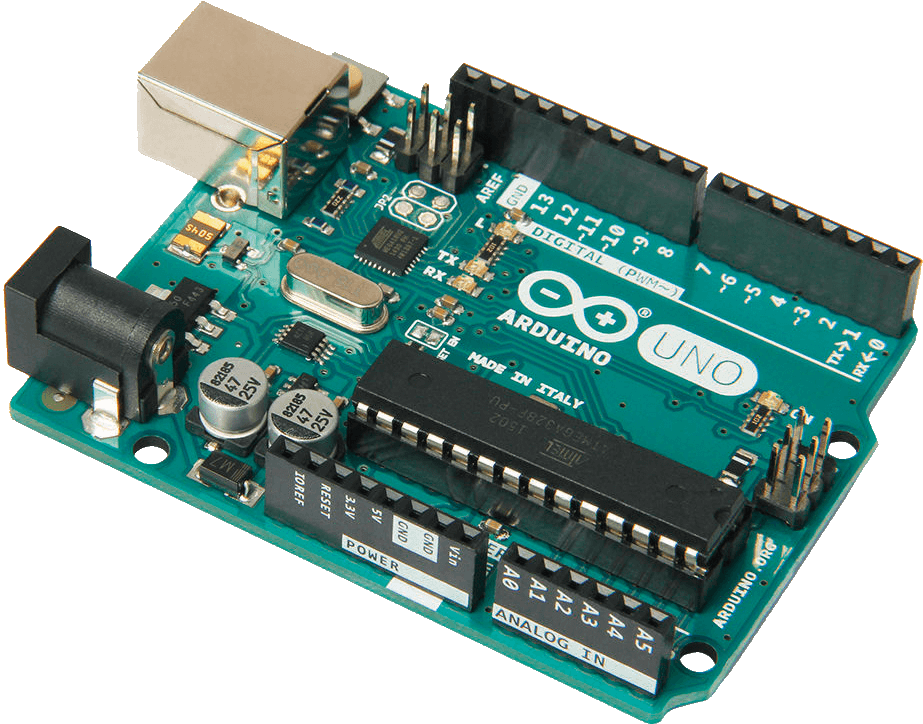
\includegraphics[scale=0.25]{images/arduino-uno-r3}};
\draw[red,*-] (0.5,-0.5) -- ++(3,0) node[right] {microcontroller};
\draw[red,*-] (-1.5,1.9) -- ++(0,.5) -- ++(2,0) node[right] {USB-connector};
\draw[red,*-] (1.5,1.3) -- ++(2,0) node[right] {headers};
\draw[red,*-] (0.0,-1.3) -- ++(3,0) node[right] {headers};
\end{tikzpicture}
\caption{Foto van een Arduino Uno met daarop een ATmega328-controller.}
\label{fig:arduinouno}
\end{figure}

Op de PCB \textsl(printed circuit board)\index{printed circuit board}\index{PCB!\see{printed circuit board}} is de microcontroller te zien (het lange, rechthoekige object). Dit is het hart van het systeem. Linksboven is een USB-connector te zien waarmee we de microcontroller kunnen programmeren en van spanning kunnen voorzien. Aan de boven- en onderkant zijn \textsl{headers}\index{headers} te zien waar we verbindingen kunnen maken met externe componenten, zoals drukknoppen en leds.

Met behulp van een programma op de PC (in dit geval de Arduino IDE, zie~\cite{arduino}), kunnen we een programma schrijven, compileren op de PC, en laden in de microcontroller. We noemen zo'n compiler een \textsl{cross compiler}\index{cross compiler} omdat we het programma niet op de PC draait maar op de microcontroller. In tegenstelling tot de gebruikelijke C-broncode, gebruikt de Arduino Uno twee specifieke functies, namelijk \lstinline|setup| en \lstinline|loop|. De functie \lstinline|setup| wordt eenmalig uitgevoerd als het programma start, de functie \lstinline|loop| wordt continu uitgevoerd zolang het programma draait. Zie listing~ \ref{cod:uno}.

\begin{lstlisting}[caption=Uitvoering op een Adruino Uno.,label=cod:uno]
void setup()
{
    /* eenmalige initialisatie */
}

void loop()
{
    /* continu uitvoeren */
}
\end{lstlisting}

We kunnen de Arduino iets zinnigs laten doen, zoals het inlezen van de stand van een pin (schakelaar) en het resultaat laten uitvoeren naar een pin (led). Dit is te zien in listing~ \ref{cod:arduinoio}. We beginnen met het defini\"eren van een aantal \textsl{pinnen}. Zie hiervoor de Arduino documentatie. Pin~7 is de input pin. Pin~13 is de output pin. De toekenningen zijn te zien in de regels~1 en~2. De variabele \lstinline|val| is een tijdelijke variabele en wordt gebruikt om de stand in te lezen en weg te schrijven.

\begin{lstlisting}[caption={Inlezen van een pin en het resultaat schrijven naar een pin.},label=cod:arduinoio]
int inPin = 7;    /* pushbutton connected to digital pin 7 */
int ledPin = 13;  /* LED connected to digital pin 13 */
int val = 0;      /* variable to store the value read*/

void setup() {
  pinMode(inPin, INPUT);    /* sets the digital pin 7 as input */
  pinMode(ledPin, OUTPUT);  /* sets the digital pin 13 as output */
}

void loop() {
  val = digitalRead(inPin);   /* read the input pin */
  digitalWrite(ledPin, val);  /* sets the LED to the button's value */
}
\end{lstlisting}

In de functie \lstinline|setup| wordt pin 7 als input bestempeld en pin~13 als output. Daarmee leggen we vast welke \textsl{richting} de pin heeft. In de functie \lstinline|loop|, die zoals eerder is vermeld continu wordt uitgevoerd, lezen we de stand van pin~7 in en schrijven dat naar pin~13. We moeten wel een schakelaar aan pin~7 en een led aan pin~13 plaatsen, die zijn niet op het Arduino-bord aanwezig.

We kunnen ip  de PC dit programma compileren en vervolgens in de microcontroller plaatsen waarna het wordt uitgevoerd zolang de spanning aanwezig is.

We hebben bij dit programma gebruik gemaakt van de functies \lstinline|pinMode|, \lstinline|digitalRead| en \lstinline|digitalWrite|. Deze functies alleen beschikbaar bij de Arduino Uno. Ze zorgen ervoor dat de programmeur niet precies hoeft te weten hoe de hardware van de microcontroller is georganiseerd. De hardware wordt als het ware geabstraheerd. Er zijn meer functies beschikbaar zoals het inlezen van de analoog-digitaal-converter. Als deze functies zijn samengebracht in de \textsl{Hardware Abstraction Layer} (HAL)\index{HAL}\index{Hardware Abstraction Layer} en wordt standaard geladen bij compilatie.

Overigens zijn de functies \lstinline|setup| en \lstinline|loop| als volgt te simuleren op een PC:

\begin{lstlisting}[caption=Simulatie van de functies \texttt{setup} en \texttt{loop}.]

int main(void)
{
    setup();

    while (1)
    {
        loop();
    }
}
\end{lstlisting}

De functie \lstinline|main| is te zien als functie die aangeroepen wordt door het systeem. Daarna wordt in regel 4 eenmalig de functie \lstinline|setup| aangeroepen. De functie \lstinline|loop| wordt herhaaldelijk aangeroepen in de functie \lstinline|main|.

\section{AVR ATmega}
Op de Arduino Uno R3 wordt de ATmega328 microcontroller van Microchip gebruikt~\cite{atmega328p}. Deze controller is ook te gebruiken zonder de Arduino-omgeving, maar dan is de HAL niet beschikbaar. Er zijn wel ontwikkelingsborden zoals de STK500~\cite{stk500}. Daarop kan de ATmega328 geplaatst worden. Programmeren kan via de ISP (In-circuit Serial Programming) of via de JTAG-interface. Deze laatste interface kan ook gebruikt worden voor debuggen op de chip, iets wat niet met de Arduino Uno kan.

Zoals gezegd is de HAL van de Arduino Uno niet beschikbaar, dus moeten alle functies zelf geschreven worden.







\zhlipsum[2-8]





\printbibliography
\appendix
\frontmatter



%%%%%%%%%%%%%%%%%%%%%%%%%%%%%%%%%%%%%%%%%%%%%%%%%%%%%%%%%%%%%%%%%%
%%%
%%%       INDEX
%%%
%%%%%%%%%%%%%%%%%%%%%%%%%%%%%%%%%%%%%%%%%%%%%%%%%%%%%%%%%%%%%%%%%%


%% Add index to toc with clickable reference
\cleardoublepage
\phantomsection
\addcontentsline{toc}{chapter}{\indexname}
% Next doesn't work with imakeidx, use \indexsetup{othercode=\thispagestyle{fancy}}
%\thispagestyle{fancy}

%% Just a nice trick to get ``recursie'' in the index, pointing to itself ;-)
\newcommand{\indexownpage}[1]{\textcolor{bookcolor}{\thepage}}
\printindex\index{recursie|indexownpage}


\end{document}